\documentclass[fontsize=12pt,paper=a4,twoside]{scrartcl}

\newcommand{\grad}{\ensuremath{^{\circ}} }
\renewcommand{\strut}{\vrule width 0pt height5mm depth2mm}

\usepackage[utf8]{inputenc}
\usepackage[final]{pdfpages}
% obere Seitenränder gestalten können
\usepackage{fancyhdr}
\usepackage{moreverb}
% Graphiken als jpg, png etc. einbinden können
\usepackage{graphicx}
\usepackage{stmaryrd}
% Floats Objekte mit [H] festsetzen
\usepackage{float}
% setzt URL's schön mit \url{http://bla.laber.com/~mypage}
\usepackage{url}
% Externe PDF's einbinden können
\usepackage{pdflscape}
% Verweise innerhalb des Dokuments schick mit " ... auf Seite ... "
% automatisch versehen. Dazu \vref{labelname} benutzen
\usepackage[ngerman]{varioref}
\usepackage[ngerman]{babel}
\usepackage{ngerman}
% Bibliographie
\usepackage{bibgerm}
% Tabellen
\usepackage{tabularx}
\usepackage{supertabular}
\usepackage[colorlinks=true, pdfstartview=FitV, linkcolor=blue,
            citecolor=blue, urlcolor=blue, hyperfigures=true,
            pdftex=true]{hyperref}
\usepackage{bookmark}
\usepackage{enumitem}
\usepackage{pdfpages}

\newboolean{langversion} %Deklaration
\setboolean{langversion}{true} %Zuweisung ist 'false' für Blockkurs
\newcommand{\highlight}[1]{\textcolor{blue}{\textbf{#1}}}
\newcommand{\nurlangversion}[0]{%
\ifthenelse{\boolean{langversion}}{\highlight{Muss in SWP-2 ausgefüllt werden}}{\highlight{Entfällt in SWP-1}}}

\newcommand{\swp}[0]{\ifthenelse{\boolean{langversion}}%
{Software--Projekt 2}{Software--Projekt 1}}
\newcommand{\jahr}[0]{2014}
\newcommand{\semester}[0]{\ifthenelse{\boolean{langversion}}{WiSe}{SoSe} \jahr}

% Damit Latex nicht zu lange Zeilen produziert:
\sloppy
%Uneinheitlicher unterer Seitenrand:
%\raggedbottom

% Kein Erstzeileneinzug beim Absatzanfang
% Sieht aber nur gut aus, wenn man zwischen Absätzen viel Platz einbaut
\setlength{\parindent}{0ex}

% Abstand zwischen zwei Absätzen
\setlength{\parskip}{1ex}

% Seitenränder für Korrekturen verändern
\addtolength{\evensidemargin}{-1cm}
\addtolength{\oddsidemargin}{1cm}

\bibliographystyle{gerapali}

%Erhöht den Abstand zwischen den Tabellenzeilen ein wenig
\renewcommand{\arraystretch}{1.2}

% Lustige Header auf den Seiten
  \pagestyle{fancy}
  \setlength{\headheight}{70.55003pt}
  \fancyhead{}
   \fancyhead[LO,RE]{\swp\\ \semester{}
  \\Projektplan}
  \fancyhead[LE,RO]{Seite \thepage\\\slshape \leftmark\\\slshape \rightmark}

%
% Und jetzt geht das Dokument los....
%

\begin{document}

% Lustige Header nur auf dieser Seite
  \thispagestyle{fancy}
  \fancyhead[LO,RE]{ }
  \fancyhead[LE,RO]{Universität Bremen\\FB 3 -- Informatik\\
  Prof. Dr. Rainer Koschke \\TutorIn: Euer/Eure TutorIn}
  \fancyfoot[C]{}

% Start Titelseite
  \vspace{3cm}

 \begin{minipage}[H]{\textwidth}
  \begin{center}
  \bf
  \Large
  \swp{} \jahr\\
  \smallskip
  \small
  VAK 03-BA-901.02\\
  \vspace{3cm}
  \end{center}
  \end{minipage}
  \begin{minipage}[H]{\textwidth}
  \begin{center}
  \vspace{1cm}
  \bf
  {\Large Projektplan}\\
  \vspace{3ex}
  \begin{figure}[H]
  \centering
  \includegraphics[width=0.25\textwidth]{../woym.png}
  \end{figure}
  
  \vfill
  \end{center}
  \end{minipage}
  \vfill
  \begin{minipage}[H]{\textwidth}
  \begin{center}
  \sf
  \begin{tabular}{l}
  Tim Hansen \\
  Joshua Hoffmann\\
  Hassan Klait \\
  Adrian Lück \\
  Jurij Schmidt\\
  Falko Schröder
  \end{tabular}
  \\ ~
  \vspace{2cm}
  \\
  \it Version 0.9.1 \\ ~
  \end{center}
  \end{minipage}

% Ende Titelseite

% Start Leerseite

\newpage

  \thispagestyle{fancy}
  \fancyhead{}
  \fancyhead[LO,RE]{\swp{}\\ \semester{} 
  \\Projektplan}
  \fancyhead[LE,RO]{Seite \thepage\\\slshape \leftmark\\~}
  \fancyfoot{}
  \renewcommand{\headrulewidth}{0.4pt}
  \tableofcontents

\newpage

  \fancyhead[LE,RO]{Seite \thepage\\\slshape \leftmark\\\slshape \rightmark}


%%%%%%%%%%%%%%%%%%%%%%%%%%%%%%%%%%%%%%%%%%%%%%%%%%%%%%%%%%%%%%%%%%%%%%%%
\section*{Version und Änderungsgeschichte}

\begin{tabular}{ccl}
Version & Datum & Änderungen \\
\hline
0.9 & 24.10.2014 & Kapitel 1 bis auf 1.5 hinzugefügt\\
0.9.1 & 27.10.2014 & Kapitel 5 inkl. (vorläufigem) Gantt-Diagramm und Kap. 6 hinzugefügt\\
0.9.2 & 29.10.2014 & Arbeitsprozess angepasst\\
\end{tabular}


%%%%%%%%%%%%%%%%%%%%%%%%%%%%%%%%%%%%%%%%%%%%%%%%%%%%%%%%%%%%%%%%%%%%%%%%
\section{Einleitung}

\subsection{Projektübersicht}

\subsubsection{Ziele}

Ziel des Projektes ist es, eine auf Java basierende Stundenplansoftware als lokale Webapplikation für die Ganztagsschule an der Oslebshauser Heerstraße in Bremen zu entwickeln, so dass diese die Stundenpläne nicht mehr per Hand anfertigen müssen. Die Software soll die Lehrer lediglich bei dem Prozess der Stundenplananfertigung unterstützen und diesen damit effektiver und effizienter machen, nicht aber die Stundenpläne automatisch erzeugen. \\
Das System wird den Lehrern erlauben Lehrer, Klassen, Schulfächer und Räume zu erstellen, Stundenpläne für jeden Lehrer und jede Klasse anzeigen zu lassen und diesen Aktivitäten hinzuzufügen. \\
Zu den unterstützenden Funktionen zählen z.B. Warnmeldungen, wenn das Stundenkontingent eines Lehrers überschritten wird oder ein Lehrer für denselben Zeitpunkt doppelt eingetragen werden soll. \\
Die Software ist für die eher langfristige Planung der Stundenpläne für mehrere Monate gedacht, nicht für kurzfristige Veränderungen wie z.B. beim Entwerfen von Vertretungsplänen.

\subsubsection{Hauptarbeitsaktivitäten und --produkte}
\begin{tabularx}{\textwidth}{|X|X|}
\hline \textbf{Aktivität} & \textbf{Produkt}  \\ 
\hline Erstellen des Projektplans & Projektplan \\ 
\hline Erstellen der Anforderungsspezifikation & Anforderungsspezifikation \\
\hline Erstellen der Architekturbeschreibung & Architekturbeschreibung \\
\hline Erstellen des Testplans und der Blackboxtests & Testplan und Blackboxtests \\
\hline Implementierung & Die Software gemäß der zuvor entworfenen Dokumente. \\
\hline 
\end{tabularx} 

\clearpage
\subsubsection{Haupt--Meilensteine und grober Zeitplan}

\begin{tabularx}{\textwidth}{|p{5cm}|p{2cm}|X|}
\hline \textbf{Meilenstein} & \textbf{Datum} & \textbf{Kriterien zur Erfüllung} \\
\hline Projektplan fertiggestellt & 29.10.2014 & Alle Kapitel sind vollständig. \\
\hline Anforderungsspezifikation fertiggestellt & 05.11.2014 & Die Anforderungsspezifikation enthält alle wichtigen im Kundengespräch erfahrenen Anforderungen. Die Anforderungsspezifikation ist inhaltlich zutreffend, vollständig, neutral und widerspruchsfrei, sowie leicht verständlich und präzise.\\
\hline Architekturbeschreibung fertiggestellt & 18.11.2014 & Es wurde eine globale Analyse nach Hofmeister durchgeführt. Die Architektur ist gründlich und präzise dargelegt und aus konzeptioneller, Modul-, Daten- und Ausführungssicht dargestellt.   \\
\hline Testplan und Blackboxtests fertiggestellt & 29.11.2014 & Der Testplan sowie alle darin aufgeführten Blackboxtests sind fertiggestellt.\\
\hline Programmiertechnische Fertigstellung des Projektes & 23.01.2015 & Das Projekt erfüllt alle Mindestanforderungen, ist lauffähig und erreicht die im Testplan spezifizierten Testabdeckungen.\\
\hline Endgültige Abgabe des Projektes & 08.02.2015 & Benutzerhandbuch, Architekturbeschreibung, Testprotokoll und kommentierter Quelltext mit maven-Build-Skript werden abgegeben. \\
\hline
\end{tabularx}

\subsubsection{Kontaktdaten des Kunden}
GTS Oslebshauser Heerstraße \\
Oslebshauser Heerstraße 115\\
28239 Bremen \\


\subsection{Auszuliefernde Produkte}
Die Software wird auf einem USB-Stick oder einer CD-Rom inkl. Installationsskript und Handbuch ausgeliefert. Das Handbuch wird dem Kunden zusätzlich in ausgedruckter Form übergeben. 

\subsection{Evolution des Plans}
Der Plan wird verändert und angepasst, wenn neue Risiken das Projekt bedrohen oder Probleme mit der Zeitplanung vorhanden sind, also beispielsweise ein Termin nicht eingehalten werden kann. Zudem wird immer die nächste folgende Projektphase im Projektplan detaillierter aufgenommen.

\subsection{Referenzen}
% mit \nocite kann man Literatur auflisten, die im Text nicht explizit
% erwähnt ist. \nocite{*} zitiert dann das ganze .bib-File
%
% Die Bibliographie erzeugt man indem man erst
%
% pdflatex bericht.tex
% bibtex bericht
% pdflatex bericht.tex
% pdflatex bericht.tex
%
% benutzt
%\nocite{Knudsen1}
%\nocite{*}
%\bibliography{literatur}

% Das renewcommand verhindert dass für die Literatur eine section* angelegt wird.
% auftaucht
{\renewcommand\section[2]{}
\bibliography{referenzen}
}

\subsection{Definitionen und Akronyme}


\section{Projektorganisation}

\subsection{Prozessmodell}
  \begin{figure}[H]
  	\centering
  	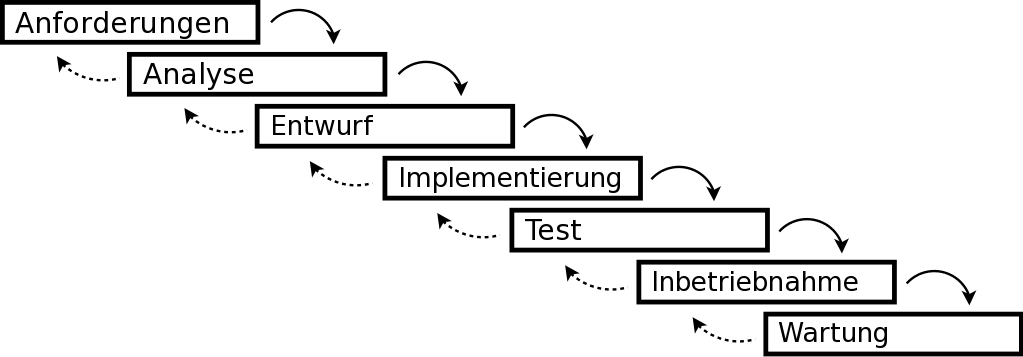
\includegraphics[width=1\textwidth]{../modell.png}
  \end{figure}
  
  Innerhalb der Implementierung ist das Modell zu beachten, das in der Issue-Tracker-Software definiert wurde.\\
  Jeder Arbeitsschritt wird hierbei von einer Person bearbeitet, eine Weitere überprüft den geschriebenen Quellcode noch einmal kritisch und danach wird eine Funktionalität in die laufende Version aufgenommen.\\
  Es wird grundsätzlich mit eigenen Kopien des Projektes gearbeitet, erst nach einem erfolgreichen Review wird eine Funktionalität eingebunden.
  \\[1\baselineskip]
  Bei der Implementierung wird nach dem \textit{Test-First}-Prinzip gearbeitet.
  

\subsection{Organisationsstruktur}

\subsubsection{Teamtreffen}

	Regelmäßige Teamtreffen sind für wöchentlich Mittwochs, 12:00Uhr MESZ im MZH der Universität geplant.\\

\subsubsection{Services}
	\textbf{Repository}\\ 
	Das Hauptrepository ist auf \textbf{GitHub} gehostet.\\
	\url{https://github.com/WOYM/timetable}
	 \\[1\baselineskip]
	 
 	\textbf{Team-Kommunikation}\\ 
	Die Kommunkation erfolgt über den Dienst \textbf{Slack}.\\
	Der dortige Channel \#general ist für allgemeine, projektbezogene Diskussionen gedacht, in den Channel \#coderelated wird Travis-CI bei Commits und Push/Pull-Requests im Repository posten. Dies dient zur Übersicht, die Diskussion von Commits, Push/Pull-Requests und Issues erfolgt zentral über den Issuetracker.\\
 	\url{https://woym.slack.com}
 	\\[1\baselineskip]
	  
	\textbf{Continous Integration}\\ 
	Das Bauen des Projektes wird von \textbf{Travis CI} übernommen.\\
	Der Dienst wird nach jedem Push/Pull-Request das Programm auf einer Ubuntu-VM durchbauen und alle JUnit-Tests laufen lassen. Bei einem Fehlschlag wird derjenige, dessen Commit zu dem Fehlschlag geführt hat per E-Mail benachrichtigt.\\
	\url{https://travis-ci.org/WOYM/timetable}
	\\[1\baselineskip]
	
	\textbf{Issue Tracker}\\ 
	Die Features und Fehler des Programmes werden über den Issue Tracker \textbf{Waffle} koordiniert. Dies ist die wohl wichtigste Anlaufstelle während des Projektes.\\
	Auf diesem Issue Tracker basiert der nachfolgend beschriebene Arbeitsprozess selbst.\\
	\url{https://waffle.io/woym/timetable}
	\\[1\baselineskip]
  
	
	\textit{\textbf{Anmerkung:} Alle der oben genannten Dienste sind (mit Ausnahme von Slack) öffentlich zugänglich und einsehbar. Private (projektintern oder auf die Person bezogen) Daten sollten nur persönlich oder über Slack weitergegeben werden. Dies gilt auch für Datenbank-Passwörter, etc. Es sind bitte immer Versionen mit Passwörtern zu commiten, die so im Live-System niemals Verwendung finden werden.}

\subsection{Verantwortlichkeiten}
	
	\textit{\textbf{Anmerkung:} Benutzernamen}\\
	
	\textbf{Datenbank}\\
	alueck\\
	hklait\\
	
	\textbf{GUI}\\
	tihansen\\
	fa\_sc\\
	
	\textbf{Logik}\\
	jur\_sch\\
	joho\\
	
	\textbf{Management}\\
	Das Management wird von allen Teammitgliedern zu gleichen Teilen bestimmt
	

\section{Managementprozess}

\subsection{Managementprozess und --prioritäten}

	Der Managementprozess basiert zum größten Teil auf der Struktur die im \textbf{Issue-Tracker} dargestellt wurde.\\
	Danach teilt sich der Prozess immer in die Elemente \textit{Planung}, \textit{Bearbeitung} und \textit{Review/Test} auf.\\
	Während der wöchentlichen Teamtreffen werden wichtige Punkte diskutiert und priorisiert.\\
	Diese Punkte werden danach für die jeweilige folgende Woche als zu bearbeitende Aufgaben festgelegt und werden nach Priorität absteigend bearbeitet.\\
	Kommunikation zu Problemen und Fehlern findet sofort über \textbf{Slack} statt, neue Ideen oder Baustellen die sich während der Implementierung auftun werden zunächst beim jeweiligen Treffen disktutiert.\\

\subsection{Annahmen, Abhängigkeiten und Einschränkungen}

\subsection{Risikomanagement}\label{riskmanagement}

{\em Wenn Ihr Euch entschieden habt, bestimmte vorbeugende Maßnahmen 
     durchzuführen, solltet Ihr dies deutlich kennzeichnen. Hoffentlich
     haben diese Maßnahmen dann einen Einfluss auf Eintrittswahrscheinlichkeit oder Schadenshöhe (zum Beispiel
     ist die Eintrittswahrscheinlichkeit von komplettem Datenverlust durch regelmäßige Backups deutlich 
     geringer). Daher solltet Ihr für diese Fälle dann die verringerten Werte für Eintrittswahrscheinlichkeit, 
     Schadenshöhe und Risikopotential zusätzlich angeben. }

{\em Wie werden neue Risiken erkannt/erfasst? Wer ist für was
  zuständig? Wie ist der Informationsfluss? \ldots 

Dieser Teil ist ein
  wichtiger Schwerpunkt des Projektplans und sollte daher ausführlich
  behandelt werden.}
  
	\begin{tabular}{|p{4cm}|p{4cm}|p{4cm}|}
	\hline
	\textbf{Risiko} & Wahrscheinlichkeit & Ausmaß \\
	\hline
	Verzögerung in der Implementierung & Mittel & Mittel \\
	\hline
	\multicolumn{3}{|p{12cm}|}{\textbf{Beschreibung}} \\
	\hline
	\multicolumn{3}{|p{12cm}|}{Es ist möglich, dass ein Feature unbekannte Probleme oder Fehler produziert, die den Zeitplan nach hinten verschieben können.} \\
	\hline
	\multicolumn{3}{|p{12cm}|}{\textbf{Maßnahmen}} \\
	\hline
	\multicolumn{3}{|p{12cm}|}{Ein zusätzlicher Puffer von zwei Wochen zum Ende der Bearbeitungszeit wurde eingerichtet, um eventuelle Verzögerungen aufzufangen.} \\
	\hline
	\end{tabular}
  
    \begin{tabular}{|p{4cm}|p{4cm}|p{4cm}|}
    \hline
    \textbf{Risiko} & Wahrscheinlichkeit & Ausmaß \\
    \hline
    Ausfall Mitglied & Mittel & Groß \\
    \hline
    \multicolumn{3}{|p{12cm}|}{\textbf{Beschreibung}} \\
    \hline
    \multicolumn{3}{|p{12cm}|}{Ein Gruppenmitglied fällt aus irgendeinem Grund über einen längeren Zeitraum aus.} \\
    \hline
    \multicolumn{3}{|p{12cm}|}{\textbf{Maßnahmen}} \\
    \hline
    \multicolumn{3}{|p{12cm}|}{Die Arbeit muss auf Bei einem sehr langen Ausfall ist eine Anpassung der Anforderungen möglich.} \\
    \hline
    \end{tabular}

\subsection{Projektüberwachung}\label{3.4-controlling}
{\em Wie wird der Projektstatus verfolgt? Wie stellt Ihr sicher, dass
  der Phasenleiter jederzeit über den Stand der Entwicklung informiert
  ist? Wie werden Probleme bzw. Verzögerungen frühzeitig erkannt und
  angegangen?}

\subsection{Mitarbeiter}
{\em Kompetenzen der und Anforderungen an die Mitarbeiter.}

%%%%%%%%%%%%%%%%%%%%%%%%%%%%%%%%%%%%%%%%%%%%%%%%%%%%%%%%%%%%%%%%%%%%%%%%

\section{Technische Prozesse}
\nurlangversion
\subsection{Methoden, Werkzeuge und Techniken}
\nurlangversion
\subsubsection{Entwicklungsplattform}

	\textbf{Spring-Tool-Suite} (STS)\\
	Zur Entwicklung mit JSF wird die STS empfohlen.\\
	\url{http://spring.io/tools/sts/all}

\subsubsection{Entwicklungsmethode}

	Test first.\\

\subsubsection{Programmiersprache und Bibliotheken}

	\textbf{Programmiersprache}\\
	Java 7\\
	\textbf{Plattform}\\
	Plattformunabhängig\\
	\textbf{Bibliotheken}
	\begin{itemize}
		\item JavaServerFaces 2.1
		\item PrimeFaces 5.0
		\item Log4J2
	\end{itemize}
	\textbf{Laufzeitumgebung}\\
	Tomcat 7.0.X ServletContainer\\

\subsection{Dokumentationsplan}
\nurlangversion

\subsubsection{Codingstyle}
	Checkstyle-konform.\\
	\textit{\textbf{Anmerkung:} Checkstyle-Konventionen können bei Teambesprechungen bei Bedarf diskutiert und angepasst werden}

\subsubsection{Kommentarsprache}

	Deutsch.\\

\subsubsection{JavaDoc}

	Deutsch.\\
	Formatiert nach JavaDoc-Vorschrift, das bedeutet, dass JavaDoc-Texte zunächst Checkstyle-konform und außerdem unter Verwendung der von JavaDoc vorgebenen Strukturelemente formatiert sein müssen.

\subsubsection{Begleitende Dokumentation}

\subsection{Unterstützende Projektfunktionen}
\nurlangversion
{\em Wie wird Euer Konfigurationsmanagement funktionieren? Wer ist verantwortlich? Benötigt Ihr dazu Ressourcen oder Zeit? Plant Ihr Datensicherung?}

{\em Gibt es Maßnahmen zur Qualitätssicherung? Wer ist zuständig?
  Wieviel Zeit ist dafür vorgesehen?}


%%%%%%%%%%%%%%%%%%%%%%%%%%%%%%%%%%%%%%%%%%%%%%%%%%%%%%%%%%%%%%%%%%%%%%%%

\section{Arbeitspakete, Zeitplan und Budget}

{\em Dieser Teil ist ein zweiter Schwerpunkt des Projektplans. Hier sollt Ihr die nächste Phase detailliert planen (siehe Arbeitspakete). Die weiteren Phasen sollen ebenfalls wenigstens grob geplant werden. Ein Gantt-Diagramm ist zwingend! 

Ihr sollt den Plan in der kommenden Phase auch tatsächlich benutzen -- und so
  Erfahrungen sammeln, was evtl. bei der Planung unberücksichtigt
  blieb. Bei der nächsten Zeitplanung (für die nächste Phase) bekommt
  Ihr dann evtl.\ eine noch bessere Planung hin.}

\subsection{Arbeitspakete}\label{aps}


\begin{enumerate}
\item \textbf{Anforderungsspezifikation}
	\begin{enumerate}[label={(\arabic*)}]
	\item Analyse der Ist- und Soll-Situation
	\item Entwicklung eines GUI-Prototypen
	\item (Entwicklung von Personas)
	\item Entwicklung eines Datenmodells
	\item Festlegung und Beschreibung der Anwendungsfälle und Aktionen
		\begin{enumerate}[label={(\arabic*)}]
		\item Festlegung und Beschreibung der Personal betreffenden Anwendungsfälle und Aktionen
		\item Festlegung und Beschreibung der Klassen betreffenden Anwendungsfälle und Aktionen
		\item Festlegung und Beschreibung der Schulfächer betreffenden Anwendungsfälle und Aktionen
		\item Festlegung und Beschreibung der Aktivitäten betreffenden Anwendungsfälle und Aktionen
		\item Festlegung und Beschreibung sonstiger Anwendungsfälle und Aktionen
		\end{enumerate}
	\item Beschreibung der Softwaresystemattribute
	\end{enumerate}	
\item \textbf{Architekturbeschreibung}
	\begin{enumerate}[label={(\arabic*)}]
	\item Durchführung einer globalen Analyse nach Hofmeister
	\item Definition der benötigten Schnittstellen, Klassen und Methoden
	\item Erstellung der konzeptionellen Sicht
	\item Erstellung der Modulsicht
	\item Erstellung der Datensicht
	\item Erstellung der Ausführungssicht
	\item Darstellung von Zusammenhängen zwischen Architektur und Anwendungsfällen mittels UML-Diagrammen
	\end{enumerate}
\item \textbf{Testplan und JUnit Tests}
		\begin{enumerate}[label={(\arabic*)}]
		\item Erstellen des Testplans
			\begin{enumerate}[label={(\arabic*)}]
			\item Einführung in den Testplan
			\item Systemüberblick
			\item Auflistung zu testender und nicht zu testender Merkmale
			\item Definition der Abnahme- und Testendkriterien
			\item Definition der Vorgehensweise bei den Tests
			\item Aufhebung und Wiederaufnahme der Tests
			\item Beschreibung der Hardware- und Softwareanforderungen
			\item Auflistung der Testfälle der Komponententests
			\item Auflistung und Beschreibung der Testfälle der Integrationstests
			\item Auflistung und Beschreibung der Testfälle der Funktionstests
			\item Auflistung und Beschreibung der Testfälle der Leistungstests
			\item Aufstellung eines Testzeitplans
			\end{enumerate}
		\item Erstellen der JUnit Blackbox-Tests
		\end{enumerate}
\item \textbf{Implementierung}
		\begin{enumerate}[label={(\arabic*)}]
		\item Implementierung der GUI
		\item Implementierung der Persistenzschicht
		\item Implementierung der Logik
		\end{enumerate}	
\end{enumerate}

\subsection{Zeitplan und Abhängigkeiten}
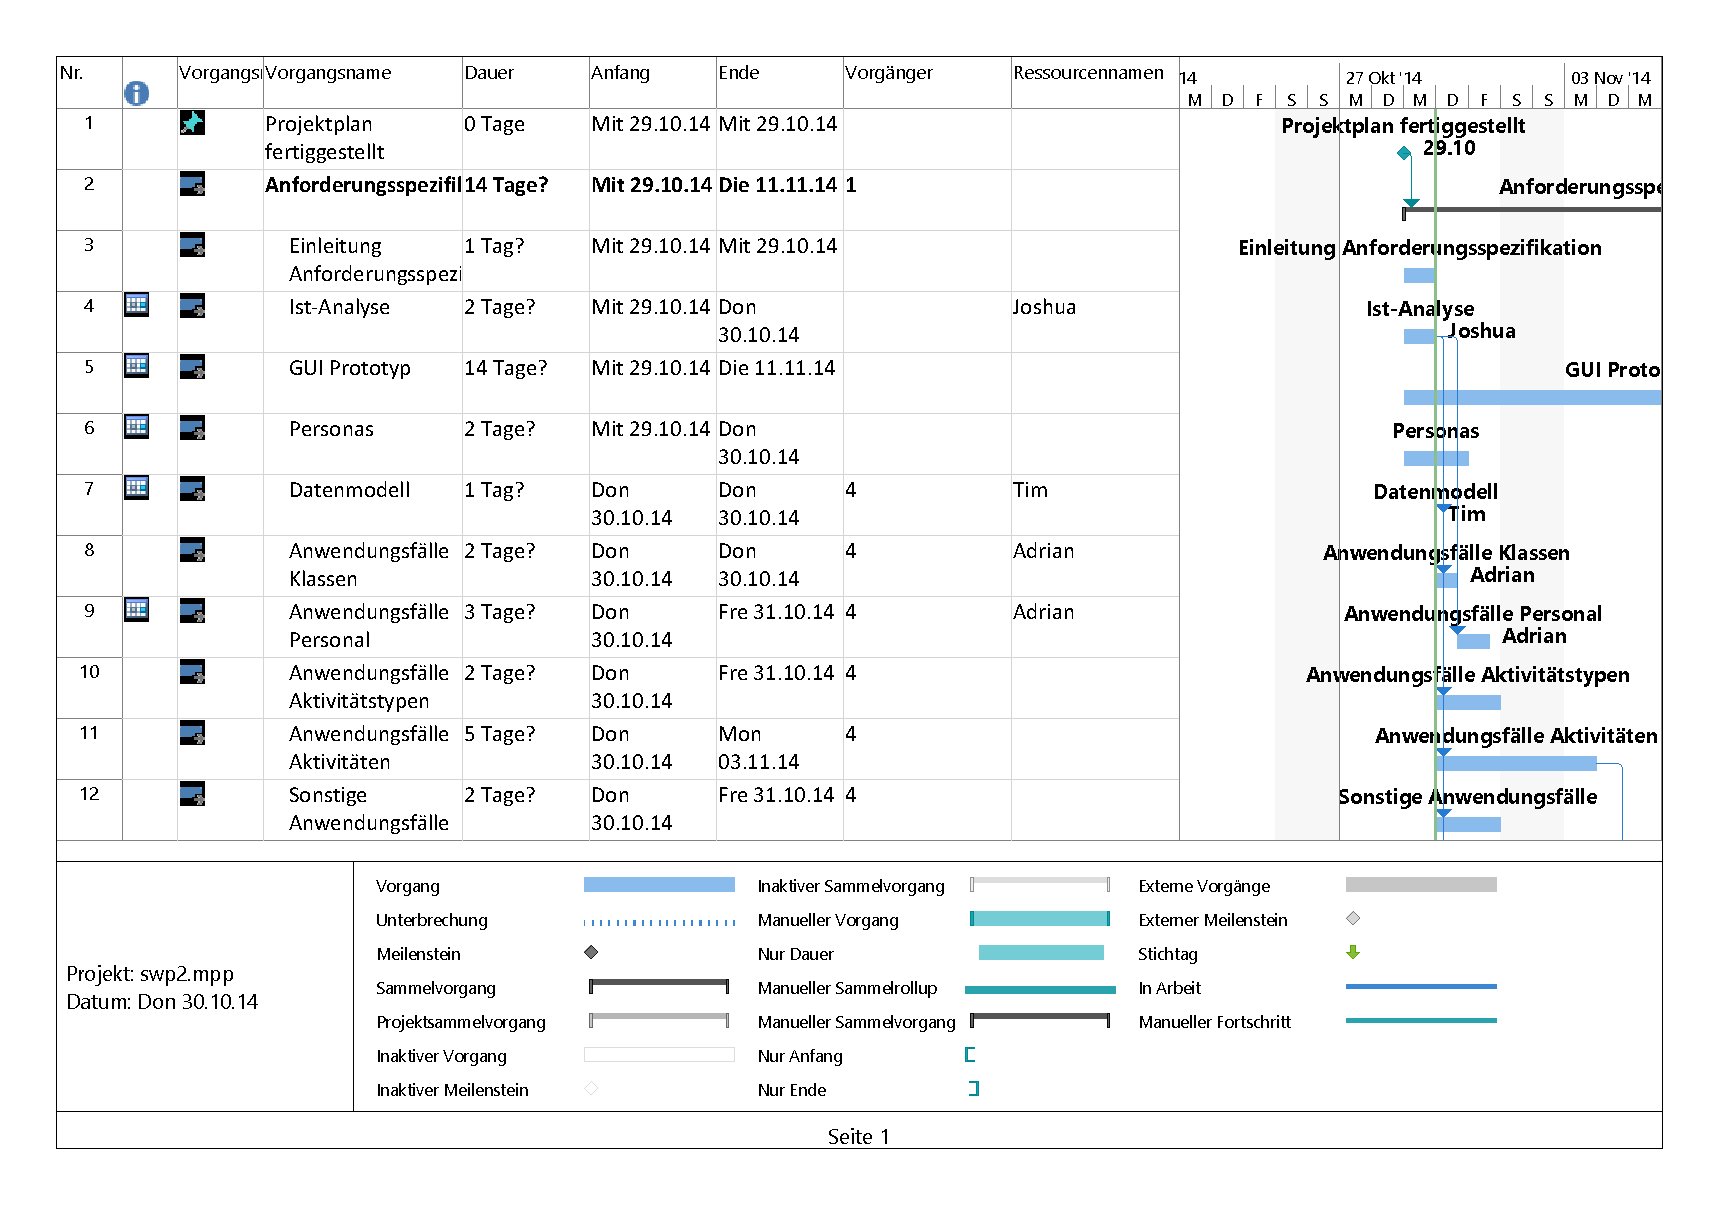
\includepdf[pages=1-12, landscape]{gantt.pdf}

\subsection{Ressourcenanforderung}

\begin{tabularx}{\textwidth}{|p{1cm}|p{5.5cm}|p{2cm}|X|}
\hline \textbf{Nr.} &\textbf{Bezeichnung} & \textbf{Dauer} & \textbf{Mitarbeiter} \\
\hline 		1.1 	& Analyse		                		&	2 Tage		&  \\
\hline 		1.2 	& GUI-Prototyp                  		&	14 Tage		&  \\
\hline 		1.3 	& Personas	                    		&   2 Tage      &  \\
\hline 		1.4 	& Datenmodell	                		&   1 Tag       &  \\
\hline 		1.5.1 	& Anwendungsfälle Personal      		&   3 Tag	    &  \\
\hline 		1.5.2 	& Anwendungsfälle Klassen       		&   2 Tage      &  \\
\hline 		1.5.3 	& Anwendungsfälle Schulfächer			&	2 Tage		&  \\
\hline 		1.5.4 	& Anwendungsfälle Aktivitäten			&	5 Tage		&  \\
\hline 		1.5.5	& sonstige Anwendungsfälle      		&	2 Tage		&  \\
\hline 		1.6 	& Softwaresystemattribute       		&	2 Tage	    &  \\
\hline		2.1		& Globale Analyse						&	4 Tage		&  \\
\hline 		2.2		& Schnittstellen, Klassen u. Methoden 	& 	4 Tage		&  \\
\hline 		2.3		& Konzeptionelle Sicht					& 	2 Tage		&  \\
\hline		2.4		& Modulsicht							&   3 Tage		&  \\
\hline 		2.5		& Datensicht							& 	2 Tage		&  \\
\hline 		2.6		& Ausführungssicht						& 	3 Tage		&  \\
\hline		2.7		& Architektur -- Anwendungsfälle		&	4 Tage		&	\\
\hline		3.1.1	& Einführung Testplan					& $\frac{1}{2}$ Tag & \\
\hline 		3.1.2	& Systemüberblick						&   1 Tag		&  \\
\hline 		3.1.3	& Merkmale								&	1 Tag		&	\\
\hline 		3.1.4	& Abnahme- und Testendkriterien			&	1 Tag		&	\\
\hline 		3.1.5	& Vorgehensweise						&	1 Tag		&	\\
\hline 		3.1.6	& Aufhebung und Wiederaufnahme			& $\frac{1}{2}$ Tag	&	\\
\hline 		3.1.7	& Hardware- und Softwareanforderungen	&$\frac{1}{2}$ Tag	&	\\
\hline
\end{tabularx}\clearpage

\begin{tabularx}{\textwidth}{|p{1cm}|p{5.5cm}|p{2cm}|X|}
\hline 		3.1.8	& Testfälle Komponententests			&	1 Tag		&	\\
\hline 		3.1.9	& Testfälle Integrationstests			&	4 Tage		&	\\
\hline		3.1.10  & Testfälle Funktionstests				&	4 Tage		&	\\
\hline 		3.1.11	& Testfälle Leistungstests				&	2 Tage		&	\\
\hline 		3.1.12	& Testzeitplan							&	2 Tage		&	\\
\hline 		3.2		& Blackbox-Tests						&	4 Tage		&	\\
\hline 		4.1		& Implementierung GUI					&	55 Tage		&	\\
\hline 		4.2		& Implementierung Persistenzschicht		&	55 Tage		&	\\
\hline 		4.3		& Implementierung Logik					&	55 Tage		&	\\	
\hline
\end{tabularx}
\clearpage

%%%%%%%%%%%%%%%%%%%%%%%%%%%%%%%%%%%%%%%%%%%%%%%%%%%%%%%%%%%%%%%%%%%%%%%%
\section{Sonstige Elemente}

\subsection{Installationspläne}
Die Installation erfolgt mithilfe eines Installationsskripts, welches zunächst einen Tomcat-Server auf dem System und anschließend die mit maven gebaute Webapplikation installiert. Ein Shortcut zum Aufruf dieser wird auf dem Desktop angelegt. 

\end{document}
